\documentclass[11pt,a4paper]{article}

\usepackage[utf8]{inputenc}
\usepackage[T1]{fontenc}
\usepackage{amsmath,amssymb,graphicx,booktabs,float,geometry,xcolor,hyperref}
\geometry{margin=2.3cm}
\newcommand{\ok}{\textcolor{green!50!black}{\textbf{anda}}}
\newcommand{\no}{\textcolor{red!70!black}{\textbf{no anda}}}
\title{Experimentos exploratorios: Laplaciano en la L y $p$-Laplaciano con $p=3.5$}
\author{Informe interno (fuera de la revisión)}
\date{18 de noviembre de 2026 --- estado preliminar}
\renewcommand{\figurename}{Figura}\renewcommand{\tablename}{Tabla}\renewcommand{\abstractname}{Resumen}
\begin{document}
\maketitle

\begin{abstract}
Dos ejemplos que no habían funcionado en versiones anteriores del método: (i) el Laplaciano de Dirichlet en el dominio en L
$\Omega=[-1,1]^2\setminus[0,1]^2$ (y la cruz con $a=1/4$), y (ii) el $p$-Laplaciano con $p=3.5$ en el disco unidad.
\textbf{L:} imponiendo Dirichlet con $u=B(x)\,\mathrm{NN}$ el entrenamiento oscila y no converge (se reproduce la
inestabilidad observada por los autores); imponiendo la condición de borde en forma \emph{débil} (penalización en la loss)
la curva de loss es suave, detecta los tres autovalores de $[6,25]$ sin espurios y da $E_1,E_2,E_3$ con diferencias
$-2.1\%$, $-0.02\%$, $-0.7\%$ respecto de FEM. \textbf{Cruz:} no funciona con ninguna variante probada.
\textbf{$p=3.5$:} el método base detecta $E_1$, pero la curva es plana y el valor depende del nodo
($\pm1$--$2\%$); una entrada singular $|x|^{p/(p-1)}$ en la red baja la loss un orden de magnitud y da $E_1$ con $\le0.3\%$
en tres semillas. El segundo autovalor ($\approx69.16$) \emph{no} se obtiene.
Todo es una sola corrida (o tres semillas donde se indica), en CPU.
\end{abstract}

\section*{Resumen: qué anda y qué no}
\begin{center}
\begin{tabular}{p{6.3cm}p{1.6cm}p{6.6cm}}
\toprule
Experimento & Estado & Comentario\\
\midrule
L, Dirichlet fuerte $u=B\,\mathrm{NN}$ & \no & residuo oscila entre 25 y 90 sin converger (4 variantes de $B$)\\
L, Dirichlet débil, $\beta=100$--$300$ & \ok & curva suave, 3 mínimos correctos, $E_1$ con $-2\%$\\
L, Dirichlet débil, $\beta=10^4$ & \no & colapso $u\equiv0$\\
Cruz $a=1/4$, Dirichlet fuerte (12 variantes) & \no & colapso $u\equiv0$\\
Cruz, Dirichlet débil & \no & no colapsa pero viola el borde (29\% de la masa)\\
$p=3.5$, $E_1$, método base & \ok\ (parcial) & detecta $E_1$; valor depende del nodo, $\pm1$--$2\%$\\
$p=3.5$, $E_1$, entrada singular & \ok & loss $\times\frac1{10}$, $E_1$ con $-0.3\%$ a $+0.2\%$ (3 semillas)\\
$p=3.5$, $E_1$, formulación mixta & \ok\ (parcial) & entrenamiento muy estable, misma precisión que la base\\
$p=3.5$, $E_2$ & \no & colapso casi siempre; un solo nodo da 69.39 (indicio)\\
\bottomrule
\end{tabular}
\end{center}

%==========================================================
\section{Laplaciano de Dirichlet en la L}

\subsection{Planteo}
$\Omega=[-1,1]^2\setminus[0,1]^2$, $-\Delta u=Eu$, $u=0$ en $\partial\Omega$, $V=0$. La esquina reentrante (ángulo $3\pi/2$)
está en el origen; allí las autofunciones tienen una parte singular $c\,r^{2/3}\sin(2\theta/3)$, que está en $H^1_0$ pero
\emph{no} en $H^2$.

\paragraph{Referencia FEM.} Elementos $P_2$ con refinamiento graduado hacia la esquina:
$E_1=9.6402$ (valor conocido $9.6397$), $E_2=15.1984$, $E_3=19.7424$, $E_4=29.5307$, $E_5=31.9246$.

\paragraph{Red y loss.} MLP $3\times128$ tanh, Adam, Monte Carlo con 5000 puntos interiores (nuevos en cada época).
Dos maneras de imponer el borde:
\begin{itemize}
\item \textbf{Fuerte:} $u=B(x)\,\mathrm{NN}(x)$ con $B$ una función R que se anula en los 6 lados; loss
$\;\frac1{|\Omega|}\!\int(\Delta u+Eu)^2+\mu\big(\frac1{|\Omega|}\!\int u^2-1\big)^2$.
\item \textbf{Débil:} $u=\mathrm{NN}(x)$ sin factor, y se agrega $\beta\cdot\mathrm{media}_{\partial\Omega}(u^2)$ con 1500 puntos
en el borde.
\end{itemize}
Barrido: grilla $E=6.4,7.4,\dots,24.4$ (paso 1, desfasada a propósito respecto de los autovalores), $\mu=200$,
2000 épocas por nodo, tasa de aprendizaje $10^{-3}$ multiplicada por $0.999$ en cada época, arranque en caliente
(cada nodo parte de la red del anterior). Unos 4 minutos por nodo en un núcleo.

Para cada red entrenada se calcula, con $2\cdot10^5$ puntos nuevos:
\[
\rho_{\rm res}=\frac{-\int u\Delta u}{\int u^2},\qquad
\rho_{\rm var}=\frac{\int|\nabla u|^2}{\int u^2},\qquad
r^2=\frac{\int(\Delta u+Eu)^2}{\int u^2},\qquad
\text{viol.\ borde}=\frac{\mathrm{media}_{\partial\Omega}u^2}{\mathrm{media}_\Omega u^2}.
\]
Para $u\in H^1_0$ vale $\rho_{\rm res}=\rho_{\rm var}$; la diferencia es el término de borde $\int_{\partial\Omega}u\,\partial_nu$.

\subsection{Dirichlet fuerte: no anda}
\begin{figure}[H]\centering
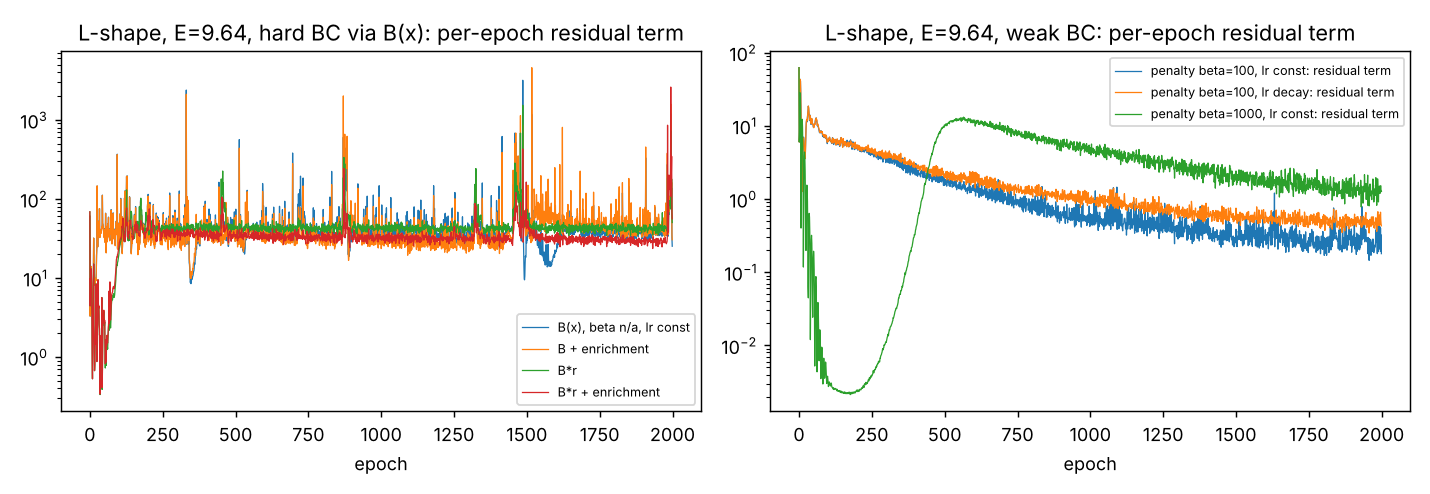
\includegraphics[width=\textwidth]{fig/L_epoch_histories.png}
\caption{Nodo único $E=9.64\approx E_1$, entrenamiento desde cero, término de residuo $\mathrm{media}(\Delta u+Eu)^2$
por época (sin normalizar por la masa). Izquierda: Dirichlet fuerte con cuatro factores
($B$; $B$ + funciones singulares exactas $r^{2/3}\sin\frac{2\theta}3$, $r^{4/3}\sin\frac{4\theta}3$ con coeficientes entrenables;
$B\cdot r$; $B\cdot r$ + singulares). Derecha: Dirichlet débil.}
\end{figure}
\begin{itemize}
\item Con $B(x)$ el residuo queda oscilando entre 25 y 90 durante 2000 épocas con picos de $10^3$, sin tendencia a bajar
($r=8.4$--$10$, masa $0.35$--$0.69$). Es la ``curva de loss que oscila'' que observaban los autores.
La caída inicial (épocas 0--50) es espuria: la red arranca con $u\approx0$.
\item \textbf{Causa de los picos:} $B$ es sólo Lipschitz en la esquina y $\Delta B\sim 1/r$; entonces $(\Delta u)^2\sim 1/r^2$
no es integrable (divergencia logarítmica) y el estimador Monte Carlo del residuo tiene varianza infinita: cuando la muestra
trae puntos muy cerca de $0$ el residuo de esa época se dispara y Adam salta. En la cruz, la misma red evaluada en 20
muestras distintas dio $r$ entre 35 y 218.
\item \textbf{Causa de fondo:} en un dominio no convexo $H^2\cap H^1_0$ no es denso en el dominio del Laplaciano de Dirichlet
con la norma del grafo, porque la parte singular $r^{2/3}\sin(2\theta/3)$ es armónica pero no $H^2$. Una red suave
multiplicada por $B$ no puede representarla, y $\inf\int(\Delta u+Eu)^2/\int u^2$ sobre esa clase queda acotado lejos de 0
incluso en un autovalor. Agregar las funciones singulares a mano y multiplicar por $r$ no alcanzó (hipótesis consistente con
los datos, no demostrada numéricamente).
\end{itemize}

\subsection{Dirichlet débil: anda}
En el panel derecho de la figura anterior el residuo baja en forma suave y monótona, con ruido Monte Carlo normal
(sin picos): la red es suave y no hay factor $1/r$. Con $\beta=1000$ la red primero casi colapsa (residuo $2\cdot10^{-3}$ con
$u\approx0$, épocas 0--200), la normalización la saca y después converge lentamente; con $\beta=10^4$ colapsa a $u\equiv0$.
Pruebas en el nodo único $E=9.64$:
\begin{center}
\begin{tabular}{lcccccc}
\toprule
$\beta$, protocolo & $\rho_{\rm res}$ & $\rho_{\rm var}$ & $r$ & masa & viol.\ borde & dif.\ vs FEM\\
\midrule
100, lr constante & 9.4606 & $9.464\pm0.035$ & 0.55 & 1.00 & $7\cdot10^{-3}$ & $-1.9\%$\\
1000, lr constante & 9.5076 & 9.491 & 1.12 & 0.99 & $2.7\cdot10^{-3}$ & $-1.4\%$\\
100, lr $\times0.999$ & 9.6055 & 9.811 & 0.68 & 0.95 & $9\cdot10^{-3}$ & $-0.4\%$\\
$10^4$, lr $\times0.999$ & \multicolumn{6}{c}{colapso (masa 0)}\\
\bottomrule
\end{tabular}
\end{center}

\subsection{Barrido en $E$ con Dirichlet débil}
\begin{figure}[H]\centering
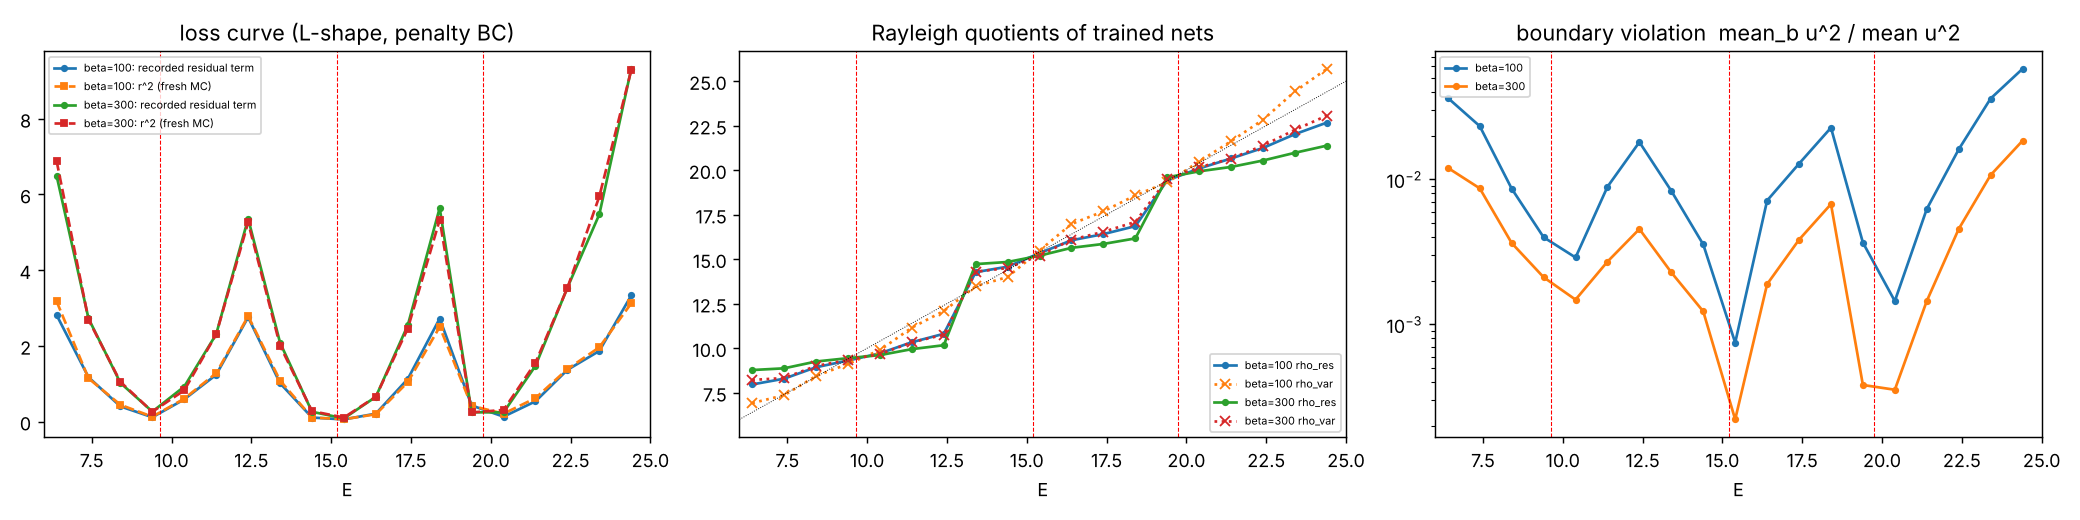
\includegraphics[width=\textwidth]{fig/L_penalty_scan.png}
\caption{Barrido $E\in[6.4,24.4]$, $\beta=100$ y $300$. Líneas rojas verticales: autovalores FEM.
Izquierda: curva de loss. Centro: cocientes de Rayleigh de las redes entrenadas (línea punteada negra: cociente $=E$).
Derecha: violación de borde.}
\end{figure}

\paragraph{Panel izquierdo (curva de loss).} Hay cuatro curvas, dos por cada $\beta$, que se superponen:
el término de residuo registrado en la última época (sobre los puntos de entrenamiento) y $r^2$ recalculado con $2\cdot10^5$
puntos nuevos. Que coincidan muestra que el valor no es un artefacto de la muestra. Los valles caen en los tres autovalores
de $[6,25]$; no hay mínimos espurios. Con $\beta=300$ la curva queda más alta entre autovalores (el borde más estricto deja
menos margen). Comparación con $\Lambda(E)=\mathrm{dist}(E,\sigma)^2$:
en $E=6.4$ y $12.4$ la loss queda \emph{por debajo} de la teoría (6.9 y 5.3 contra 10.5 y 7.6) porque la condición débil
relaja el problema (justo ahí la violación de borde es máxima); en $E=18.4$ queda \emph{por encima} (5.5 contra 1.8):
la red viene de la autofunción de $E_2$ y no llegó al ínfimo (error de optimización).

\paragraph{Panel central (cocientes).} En teoría el minimizador en $E$ es la autofunción del autovalor más cercano, así que el
cociente debería ser una escalera: $E_1$ hasta $(E_1+E_2)/2\approx12.4$, $E_2$ hasta $\approx17.5$, $E_3$ después.
Se observa la escalera, con dos diferencias: los escalones tienen pendiente (la red lejos del autovalor es una mezcla;
en $E=6.4$ el cociente 8.8 es menor que $E_1$, sólo posible violando Dirichlet) y el segundo salto llega tarde
(entre 18.4 y 19.4; histéresis del arranque en caliente). $\rho_{\rm res}$ y $\rho_{\rm var}$ coinciden cerca de los
autovalores y se separan entre ellos. \textbf{Conclusión:} el cociente sólo vale en los nodos del mínimo.

\paragraph{Panel derecho (violación de borde).} Es mínima justamente en los autovalores ($2\cdot10^{-4}$ en $E_2$ con
$\beta=300$) y máxima entre ellos; sirve como criterio de confianza.

\begin{table}[H]\centering
\caption{L, Dirichlet débil: valores en el nodo del mínimo de $r^2$. ``Parábola'': vértice de la parábola por los tres nodos
alrededor del mínimo. Una sola semilla.}
\begin{tabular}{cccccccc}
\toprule
$\beta$ & nodo & $\rho_{\rm res}$ & dif. & parábola & dif. & $r$ & viol.\ borde\\
\midrule
100 & 9.4 & 9.305 & $-3.5\%$ & 9.296 & $-3.6\%$ & 0.36 & $4\cdot10^{-3}$\\
100 & 15.4 & 15.334 & $+0.9\%$ & 15.154 & $-0.3\%$ & 0.25 & $8\cdot10^{-4}$\\
100 & 20.4 & 20.093 & $+1.8\%$ & 20.236 & $+2.5\%$ & 0.46 & $1\cdot10^{-3}$\\
\midrule
300 & 9.4 & \textbf{9.440} & $\mathbf{-2.1\%}$ & 9.482 & $-1.6\%$ & 0.51 & $2\cdot10^{-3}$\\
300 & 15.4 & \textbf{15.196} & $\mathbf{-0.02\%}$ & 15.135 & $-0.4\%$ & 0.33 & $2\cdot10^{-4}$\\
300 & 19.4 & \textbf{19.595} & $\mathbf{-0.7\%}$ & 19.887 & $+0.7\%$ & 0.49 & $4\cdot10^{-4}$\\
\midrule
FEM & & 9.6402 & & 15.1984 & & 19.7424 &\\
\bottomrule
\end{tabular}
\end{table}

\paragraph{Por qué $E_1$ es el peor.} Su autofunción es la que más peso tiene en la esquina (parte singular $r^{2/3}$),
y la condición débil deja escapar algo de masa justo allí, lo que baja el autovalor: todos los valores de $E_1$ quedan por
debajo de FEM. $E_2$ es casi exacto porque su autofunción es simétrica respecto de la diagonal y no tiene parte singular
fuerte. Lo mismo ocurre en FEM: $E_1$ es el que converge más lento con mallas uniformes. La diferencia de $E_3$ entre los
dos $\beta$ (0.5) se debe a que el mínimo cayó en nodos distintos (20.4 y 19.4).

\begin{figure}[H]\centering
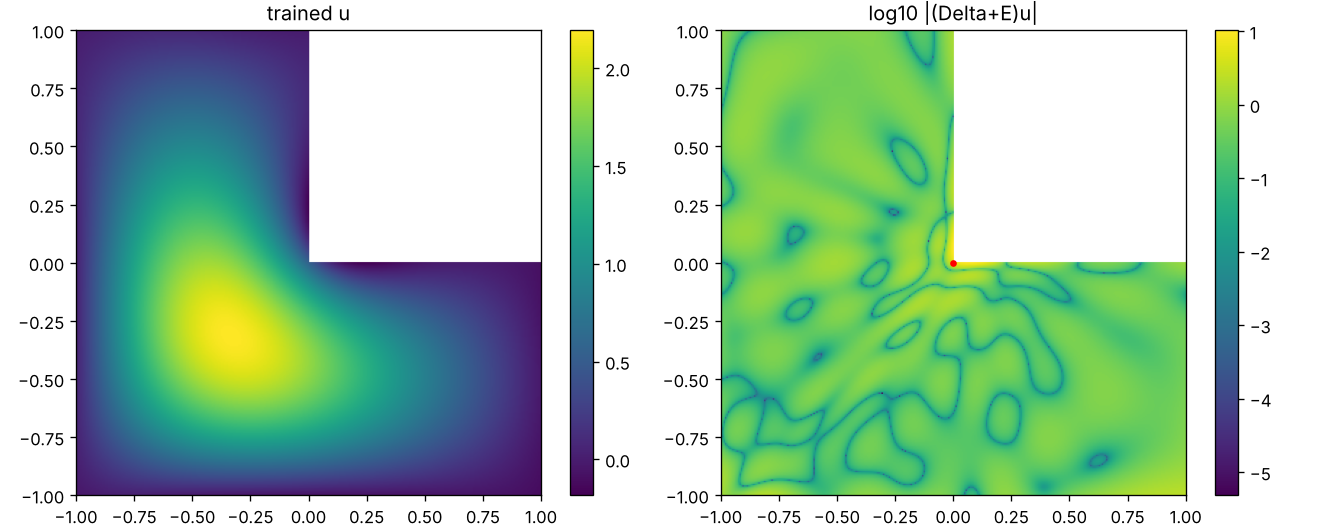
\includegraphics[width=0.85\textwidth]{fig/L_resid_pen_b100.png}
\caption{Red entrenada en $E=9.64$ ($\beta=100$). Izquierda: $u$. Derecha: $\log_{10}|(\Delta+E)u|$. El 33\% de
$\sum(\Delta u+Eu)^2$ está a distancia $<0.2$ de la esquina (3\% del área).}
\end{figure}

\subsection{Autofunciones: PINN contra FEM}
\begin{figure}[H]\centering
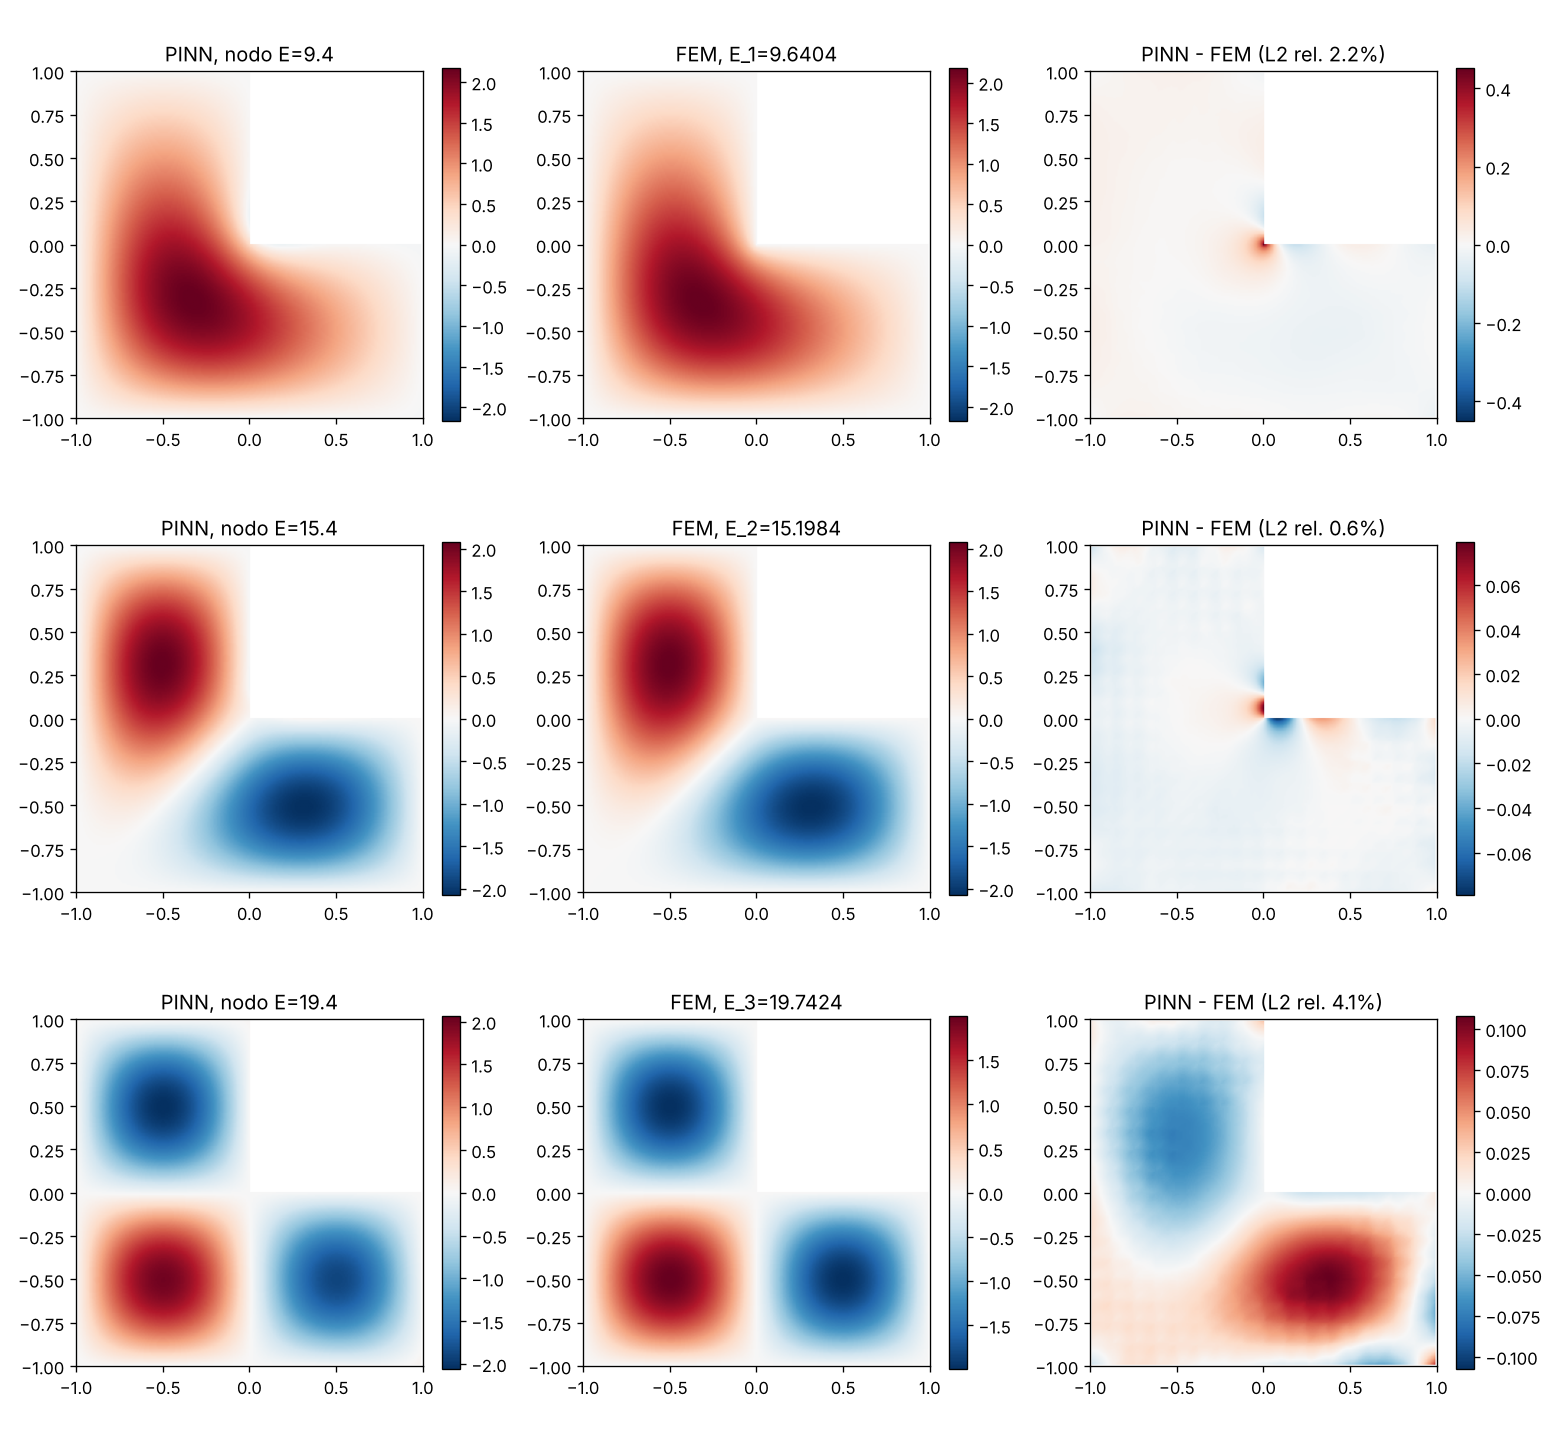
\includegraphics[width=0.92\textwidth]{fig/L_eigfun_1_2_3.png}
\caption{Autofunciones $u_1,u_2,u_3$. Izquierda: redes del barrido con $\beta=300$ en los nodos del mínimo
($E=9.4,15.4,19.4$). Centro: FEM $P_2$. Derecha: diferencia (escalas distintas en cada fila). Normalizadas en $L^2$, mismo signo.}
\end{figure}
\begin{center}
\begin{tabular}{cccccc}
\toprule
$k$ & nodo & FEM & error $L^2$ rel. & error máx.\ / máx $|u|$ & fracción del error a $<0.2$ de la esquina\\
\midrule
1 & 9.4 & 9.6404 & 2.2\% & 21\% & 54\%\\
2 & 15.4 & 15.1984 & 0.6\% & 3.8\% & 41\%\\
3 & 19.4 & 19.7424 & 4.1\% & 5.4\% & 0.4\%\\
\bottomrule
\end{tabular}
\end{center}
\begin{itemize}
\item $u_1$: el error está en la esquina reentrante (la red no reproduce $r^{2/3}$ y no se anula allí, por la condición débil);
es lo que baja $E_1$ un 2\%.
\item $u_2$: casi exacta (0.6\%); el poco error que hay también está en la esquina.
\item $u_3$: es la autofunción suave $\sin(\pi x)\sin(\pi y)$ (en la L, $E_3=2\pi^2=19.7392$ exactamente; no tiene parte
singular). El error no está en la esquina: la diferencia tiene la forma de $-u_2$, es decir, la red es $u_3$ con una
contaminación de $\approx4\%$ de $u_2$. Es la histéresis del arranque en caliente: la red viene de $u_2$, el nodo $19.4$
está a $0.34$ de $E_3$ y 2000 épocas no alcanzaron para eliminar la componente vieja. Aun así el cociente da $19.595$
($-0.7\%$), porque el cociente de Rayleigh es cuadráticamente insensible a errores en la autofunción.
\end{itemize}

\subsection{La cruz ($a=1/4$)}
FEM: $E_1=26.1149$, $E_{2,3}=48.1357$ (doble), $E_4=52.2307$, $E_5=59.0313$. Con Dirichlet fuerte colapsa a $u\equiv0$ en
las 12 variantes probadas (distintos $B$, funciones singulares, más puntos, $\mu$, lr). Con Dirichlet débil ($\beta=100$)
no colapsa, pero el 29\% de la masa queda en el borde y los dos cocientes no coinciden (26.9 contra 17.7): no es confiable.
Las cuatro esquinas reentrantes con brazos finos hacen que la parte singular pese mucho más que en la L.
\textbf{No resuelto.}

\subsection{Pendiente (en curso)}
\begin{itemize}
\item Autofunciones $u_2,u_3$ contra FEM (el barrido repetido guardando cada red todavía no llegó a esos nodos).
\item Refinamiento local (paso 0.1) con Monte Carlo graduado hacia la esquina, con y sin pesos, 2 semillas, y $\beta=1000$
para $E_1$: separar el sesgo de la condición débil de la falta de resolución.
\item Subir $\beta$ progresivamente durante el entrenamiento; cruz con entrenamiento más largo.
\end{itemize}

%==========================================================
\section{$p$-Laplaciano con $p=3.5$ en el disco unidad}

\subsection{Planteo}
$-\Delta_pu=E|u|^{p-2}u$ en el disco unidad $D\subset\mathbb R^2$, $u=0$ en $\partial D$, con $\Delta_pu=\operatorname{div}(|\nabla u|^{p-2}\nabla u)$.

\paragraph{Referencias.} $E_1=12.15465$ por shooting radial (FEM $P_1$ con minimización del cociente: 12.15464).
Segundo autovalor (una línea nodal diametral) $=$ primero del semidisco: $69.160$ (FEM $P_1$ extrapolado, orden 2.1).

\paragraph{Red y loss base.} $u=(1-|x|^2)\,\mathrm{NN}(x)$, MLP $3\times128$ tanh, $N=5000$ puntos, $\mu=200$, 1500 épocas por nodo,
Adam con lr $10^{-3}\to10^{-5}$ (coseno), arranque en caliente:
\[
\int_D\big(\Delta_pu+E\,|u|^{p-2}u\big)^2+\mu\Big(\int_D|u|^p-1\Big)^2 .
\]
El valor reportado $E_{\rm PINN}$ es el minimizador en forma cerrada en $E$ para la red congelada,
$E_{\rm PINN}=-\langle\Delta_pu,w\rangle/\langle w,w\rangle$ con $w=|u|^{p-2}u$.

\paragraph{Variantes probadas.}
\begin{itemize}
\item \textbf{(a) mixta:} una sola red con salidas $(u,\sigma)$, con $\sigma\approx|\nabla u|^{p-2}\nabla u$ (el flujo);
loss $\int(\operatorname{div}\sigma+Ew)^2+\lambda\int|\sigma-|\nabla u|^{p-2}\nabla u|^2+\mu(\cdots)^2$.
Así sólo aparecen derivadas primeras.
\item \textbf{(b) pesado hacia abajo} del residuo en el punto crítico: peso $|\nabla u|^2/(|\nabla u|^2+0.09)$;
(b$'$) dividir por $(|\nabla u|^2+0.09)^{(p-2)/2}$.
\item \textbf{(c)} más puntos ($N=20000$); muestreo por importancia (50\% de los puntos en $r<0.3$, con pesos exactos).
\item \textbf{(d)} $\mu=1000$; 5000 épocas; tasa constante con parada temprana (``P0'').
\item \textbf{(e) entrada singular:} se agrega $|x-c|^{p/(p-1)}$ como tercera entrada de la red ($c=0$ fijo o entrenable).
Es el perfil local exacto de una autofunción cerca de un máximo no degenerado
($u\approx u(0)-C|x|^{p/(p-1)}$), que una red tanh suave no representa bien.
\end{itemize}

\subsection{Dónde está la dificultad}
Para $p>2$ el operador degenera donde $\nabla u=0$, es decir en el máximo de la autofunción (el centro). Allí
$u-u(0)\sim|x|^{p/(p-1)}=|x|^{1.4}$, y $\Delta_pu$ calculado sobre una red suave tiene un error grande y localizado.
\begin{figure}[H]\centering
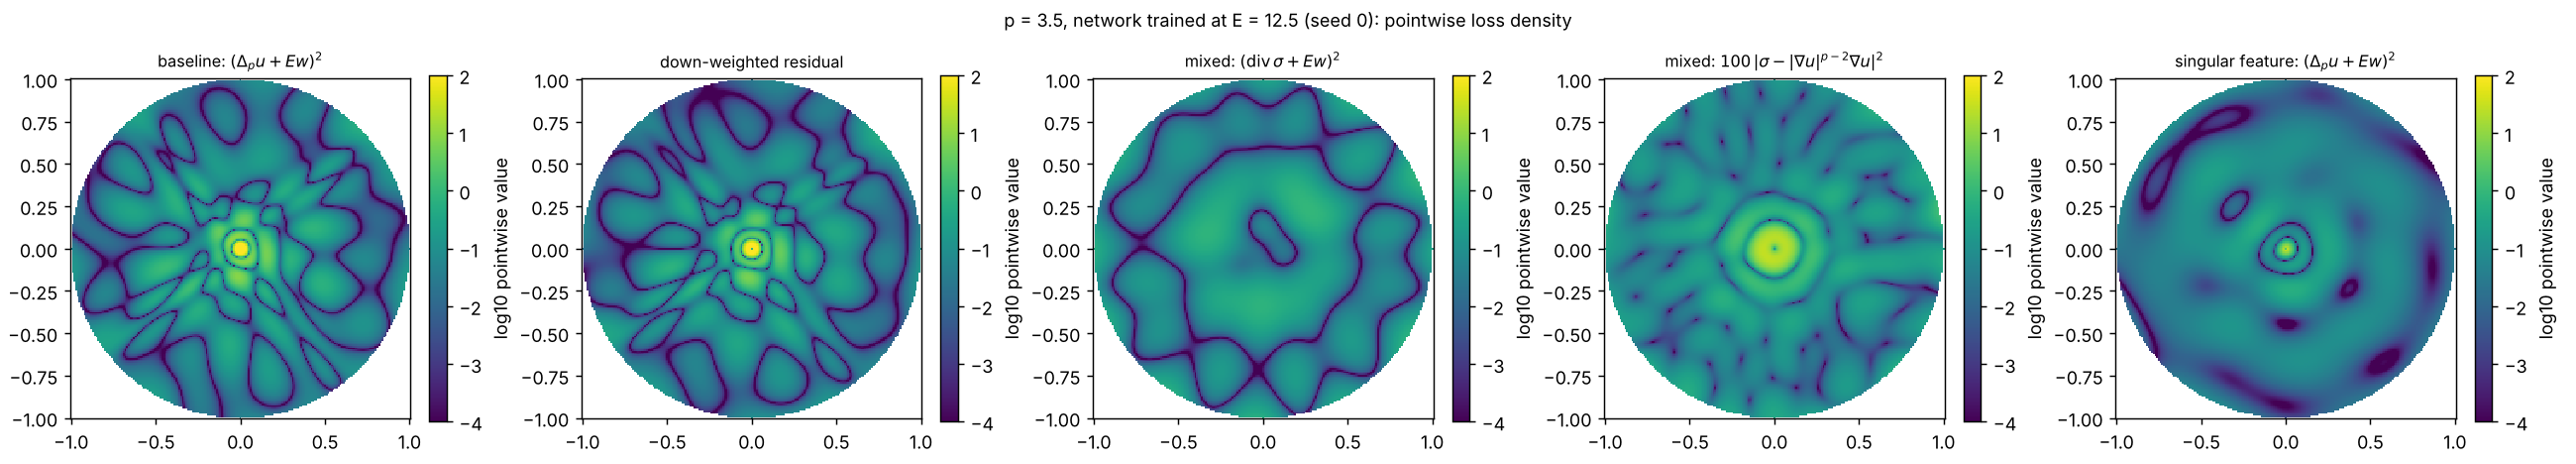
\includegraphics[width=\textwidth]{fig/p35_residual_maps.png}
\caption{Red entrenada en $E=12.5$: densidad puntual de la loss. En la base el residuo se concentra en el centro:
alrededor del 80\% de la loss está en el 2\% de puntos con menor $|\nabla u|$. Con la entrada singular (derecha) esa
fracción baja a 30\%.}
\end{figure}

\subsection{Curvas de loss}
\begin{figure}[H]\centering
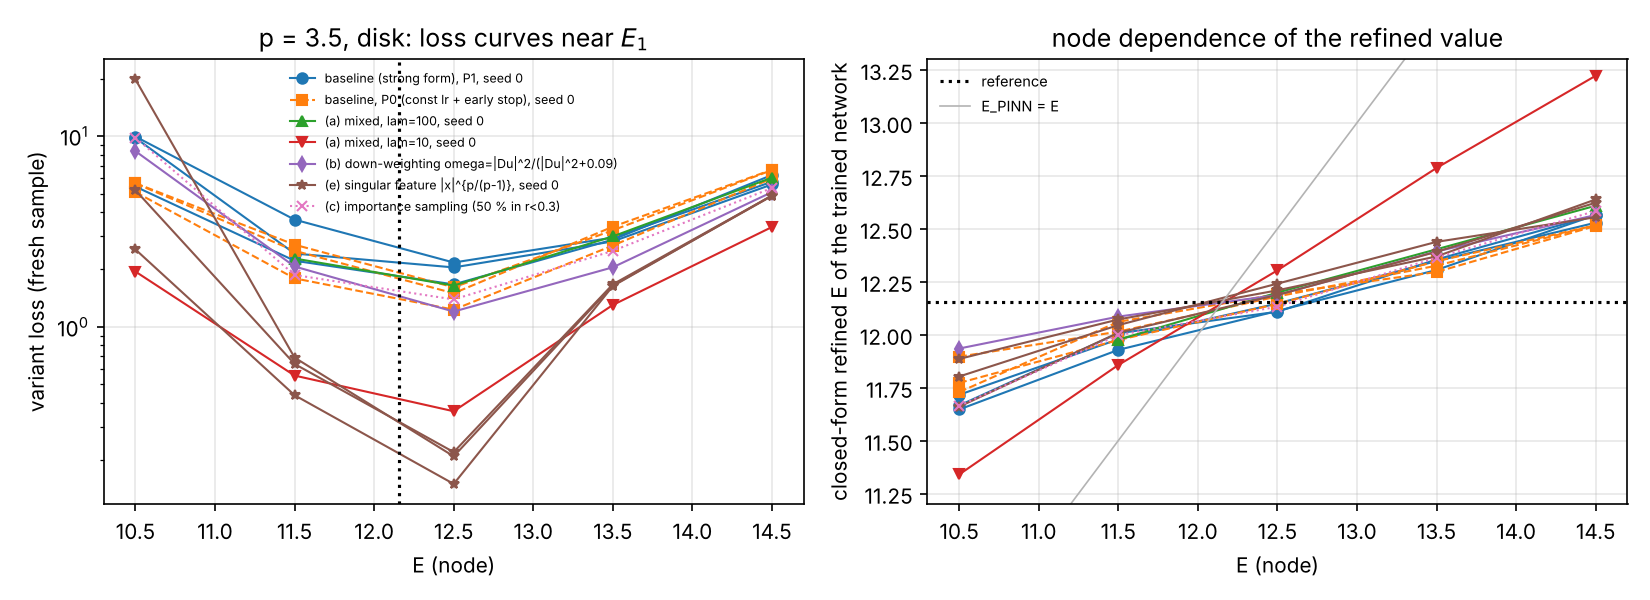
\includegraphics[width=\textwidth]{fig/p35_curves.png}
\caption{Izquierda: loss en la ventana $E=10.5,\dots,14.5$ (paso 1), evaluada con 40000 puntos nuevos; línea punteada:
referencia $E_1=12.1546$. Derecha: $E_{\rm PINN}$ de la red entrenada en cada nodo; línea gris: $E_{\rm PINN}=E$.}
\end{figure}
\begin{itemize}
\item \textbf{Todas las variantes tienen el mínimo en el nodo $12.5$}, el más cercano a $E_1$: la detección funciona.
\item \textbf{La curva base es plana:} el piso es $\approx2$ (contra 10 y 6 en los extremos), y casi todo ese piso viene del centro.
\item \textbf{El valor depende del nodo} (panel derecho): en la base, $E_{\rm PINN}$ va de 11.65 a 12.56 a lo largo de la ventana,
o sea la red no ``se queda'' en la autofunción sino que se acomoda a $E$. Donde la curva corta $E_{\rm PINN}=E$
(``punto fijo autoconsistente'' $E^*$) da una estimación independiente del nodo.
\item \textbf{Entrada singular (marrón):} la loss en $12.5$ baja a $0.15$--$0.22$, un orden de magnitud menos, y el mínimo es
mucho más marcado.
\end{itemize}

\begin{figure}[H]\centering
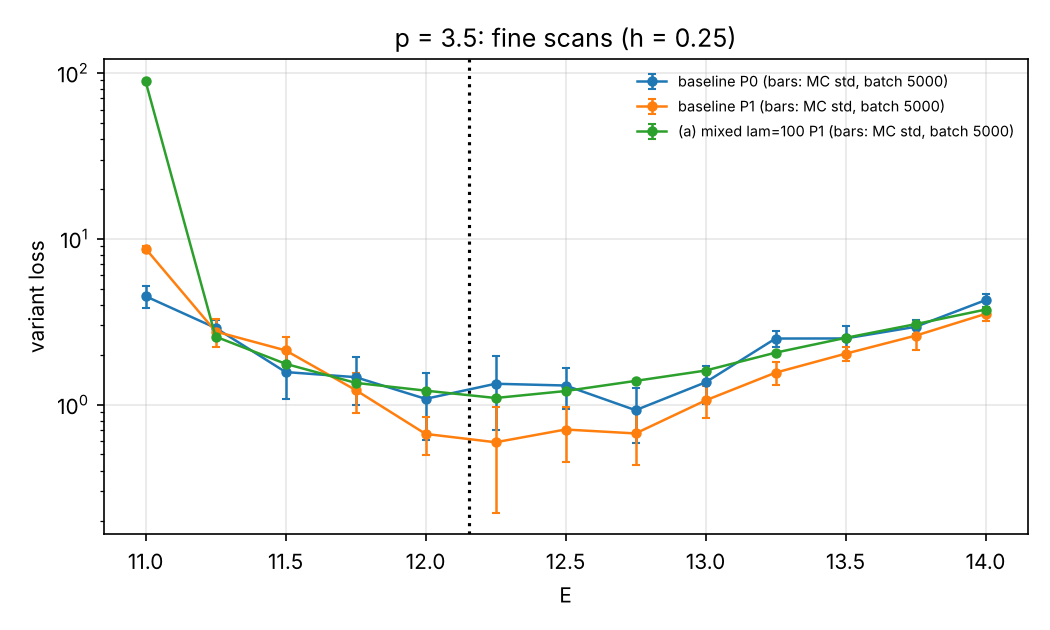
\includegraphics[width=0.7\textwidth]{fig/p35_fine_curves.png}
\caption{Barrido fino ($h=0.25$) con barras de error Monte Carlo (desvío entre lotes de 5000 puntos). En la base las
barras son comparables a la profundidad del valle: entre 12.0 y 12.75 los nodos son indistinguibles. La mixta tiene
barras despreciables pero un valle igual de plano.}
\end{figure}

\begin{figure}[H]\centering
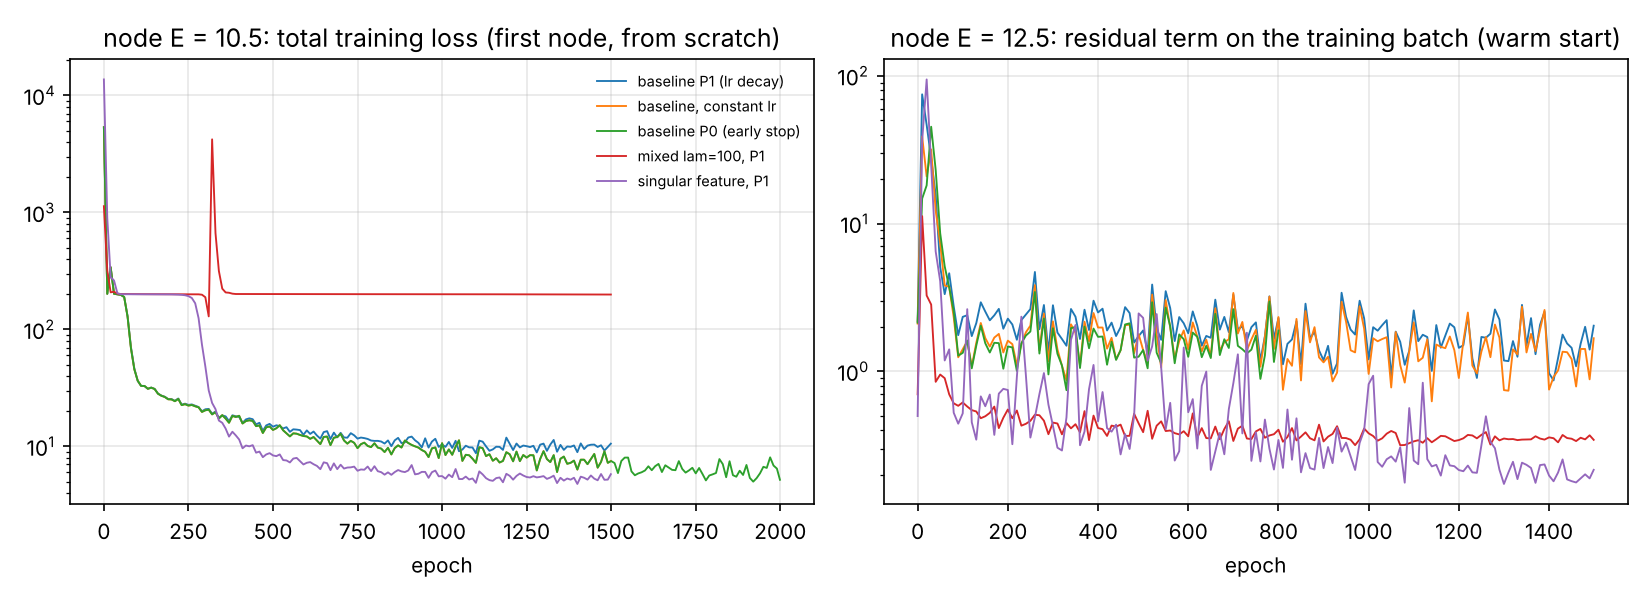
\includegraphics[width=\textwidth]{fig/p35_training_histories.png}
\caption{Historias de entrenamiento. Izquierda: primer nodo desde cero; la mixta y la entrada singular pasan cientos de épocas
en la meseta $u\approx0$ (loss $=\mu$) antes de salir. Derecha: nodo $12.5$; la base oscila (0.8--5) por el ruido de
muestreo del centro; la mixta es casi constante y la entrada singular queda en 0.2--0.5.}
\end{figure}

\subsection{Resultados para $E_1$}
\begin{table}[H]\centering
\caption{$p=3.5$, $E_1$ (referencia 12.1546). Tres semillas, nodo $E=12.5$. $E^*$: punto fijo autoconsistente.
Diferencias relativas respecto de shooting.}
\small
\begin{tabular}{lccc}
\toprule
variante & loss en 12.5 & $E_{\rm PINN}(12.5)$ & $E^*$\\
\midrule
base (lr coseno) & 2.05, 1.67, 2.17 & $-0.38,\,-0.06,\,-0.35\%$ & $-0.75,\,-0.65,\,-1.07\%$\\
base (lr const.\ + parada temprana) & 1.50, 1.23, 1.61 & $+0.30,\,+0.21,\,-0.08\%$ & $-0.08,\,-0.31,\,-0.68\%$\\
(a) mixta, $\lambda=100$ & 1.65, 1.83, 1.93 & $+0.36,\,+0.30,\,+0.23\%$ & $-0.35,\,-0.46,\,-0.89\%$\\
\textbf{(e) entrada singular} & \textbf{0.22, 0.15, 0.21} & $\mathbf{+0.71,\,+0.45,\,+0.27\%}$ & $\mathbf{+0.19,\,+0.07,\,-0.29\%}$\\
\bottomrule
\end{tabular}
\end{table}
Otras variantes (una semilla): $N=20000$, muestreo por importancia, $\mu=1000$ y pesado (b) dan lo mismo que la base
(piso $1.2$--$2.2$, $E_{\rm PINN}(12.5)$ entre $-0.5\%$ y $+0.3\%$); 5000 épocas baja la loss a $0.68$ pero no cambia la
dependencia del nodo. (b$'$) y la mixta con $\lambda=1000$ \textbf{fallan} (mínimo en el borde de la ventana,
errores de 7--19\%). La mixta con $\lambda=10$ (3 semillas) tiene loss $0.33$--$0.38$ y el vértice de la parábola de la curva
da $+0.14,\,+0.06,\,+0.22\%$, el mejor resultado de las variantes pedidas; pero su $E_{\rm PINN}$ en forma cerrada es
peor ($+0.8$ a $+1.3\%$). En \emph{todas} las variantes $E_{\rm PINN}$ se corre $\approx0.17$ por unidad de $E$ (panel
derecho de la figura anterior): a $p=3.5$ conviene leer el autovalor del mínimo de la curva estabilizada o del punto fijo
$E^*$, no del cociente en un nodo.

\paragraph{Fuentes de fluctuación} (base, $E=12.5$): ruido de muestreo de la misma red congelada
$\pm0.53$ sobre un valor de 2.05 (lotes de 5000 puntos), del mismo orden que la diferencia entre semillas (1.67--2.17).
En la mixta el ruido baja a $\pm0.008$ y con la entrada singular a $\pm0.03$. Es decir: la oscilación de la base es ruido
Monte Carlo del centro, no inestabilidad del optimizador.

\subsection{Autofunción: PINN contra shooting}
\begin{figure}[H]\centering
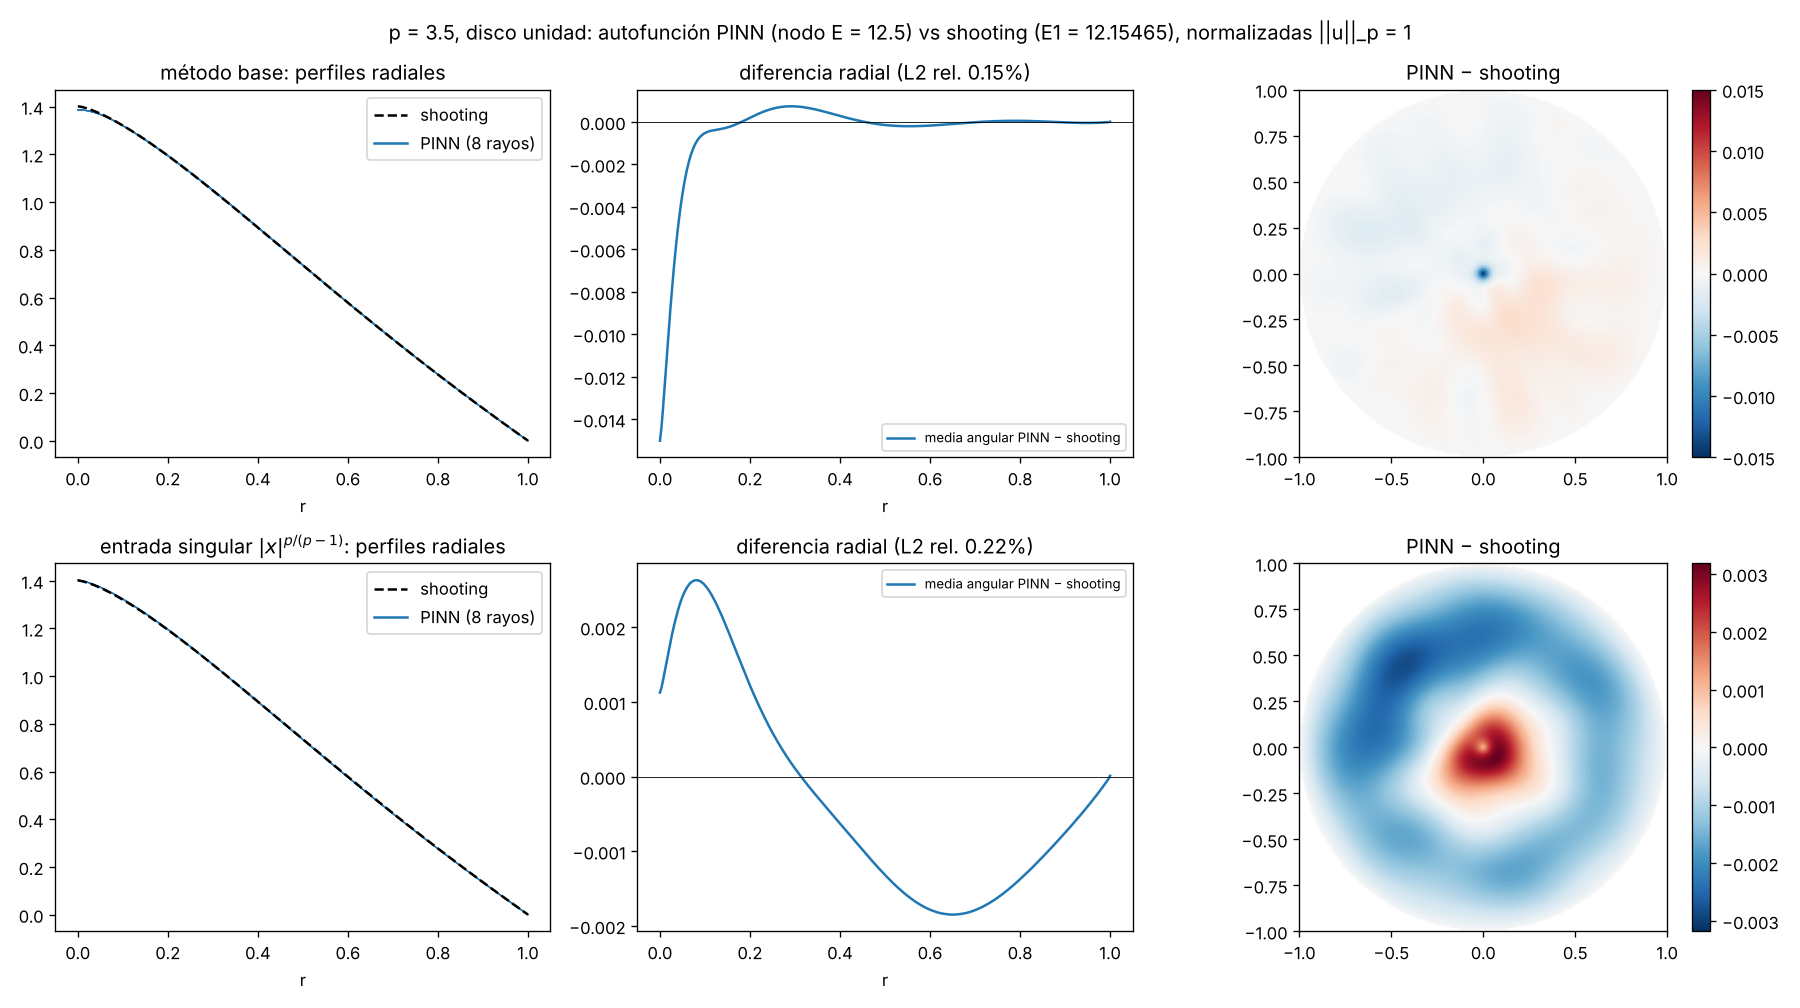
\includegraphics[width=\textwidth]{fig/p35_eigfun.png}
\caption{Primera autofunción, $p=3.5$. Arriba: método base; abajo: entrada singular. Redes entrenadas en el nodo $E=12.5$
(semilla 0); referencia: perfil radial de shooting, $u(x)=v(z_1|x|)$. Ambas normalizadas con $\|u\|_p=1$ y el mismo signo.
Izquierda: la red a lo largo de 8 rayos (azul) y shooting (negro). Centro: media angular de la diferencia en función de $r$.
Derecha: diferencia en el disco (notar las escalas distintas).}
\end{figure}
\begin{center}
\begin{tabular}{lcccc}
\toprule
variante & error $L^2$ rel. & error $L^p$ rel. & error máx.\ / máx $u$ & $u(0)$ (shooting 1.4013)\\
\midrule
base & 0.15\% & 0.22\% & 1.1\% & 1.386\\
entrada singular & 0.22\% & 0.21\% & 0.23\% & 1.402\\
\bottomrule
\end{tabular}
\end{center}
Las dos autofunciones son excelentes en norma ($\approx0.2\%$). La diferencia está en \emph{dónde} está el error:
en la base se concentra en un entorno de radio $\approx0.1$ del centro, donde la red ``achata'' el máximo ($u(0)$ un 1.1\%
bajo), justamente el punto donde $\nabla u=0$ y el operador degenera; ese error localizado es el que produce el piso de la
loss (el residuo $\Delta_pu$ es muy sensible a él). Con la entrada singular el error del centro desaparece y queda un error
suave y global de $0.2\%$, sin estructura en el punto crítico. Que la autofunción base sea buena en $L^2$ y aun así la
loss tenga un piso de 2 muestra que la loss fuerte amplifica errores locales en el punto degenerado.

\subsection{Segundo autovalor: no anda}
Ventana $E=65,\dots,73$ (referencia 69.16), redes entrenadas desde cero (3000 épocas en cada nodo):
\begin{center}
\begin{tabular}{lccc}
\toprule
corrida & masa $\int|u|^p$ en $E=65,67,69,71,73$ & loss & $E_{\rm PINN}$\\
\midrule
base & 0.007--0.06 & 880--2300 & 31--63\\
base, fijando primero la masa (500 épocas) & 0.006, 0.017, 0.23, 0.016, \textbf{0.50} & 2400, 1500, 400, 1600, \textbf{178} & 27, 48, 68, 54, \textbf{69.39}\\
mixta (con o sin fijar la masa) & 0.003--0.005 & $\approx3000$ & 14--15\\
\bottomrule
\end{tabular}
\end{center}
Casi todo colapsa a $u\approx0$: el término de normalización $\mu(\int|u|^p-1)^2$ compite con un residuo que, para una red
sin entrenar, es del orden de miles, y la solución trivial gana. Sólo el nodo $73$ con la masa fijada primero forma una
autofunción a medias (masa 0.5) con $E_{\rm PINN}=69.39$ ($+0.3\%$ respecto de 69.16): es un indicio, no un resultado.
Probablemente hace falta llegar por continuación en $E$ desde abajo (como en el caso lineal) o cambiar la normalización
o la escala inicial; no se probó.

%==========================================================
\section{Conclusiones}
\begin{enumerate}
\item \textbf{L:} la inestabilidad que se observaba viene de imponer Dirichlet con $B(x)$ en un dominio no convexo:
$\Delta B\sim1/r$ en la esquina (varianza infinita del Monte Carlo) y la parte singular $r^{2/3}$ fuera de $H^2$.
Imponiendo el borde en la loss el método funciona: curva suave, tres autovalores sin espurios, $E_2$ casi exacto y $E_1$ con
$-2\%$. El sesgo de $E_1$ es consistente con la condición débil y la singularidad de la esquina.
\item \textbf{Cruz:} sigue sin funcionar; necesita algo más (más entrenamiento, $\beta$ progresivo, o la forma débil de la
ecuación).
\item \textbf{$p=3.5$, ``oscilación'':} la loss de la base fluctúa por varianza del Monte Carlo concentrada en el centro
(la misma red congelada da $2.05\pm0.53$ entre lotes de 5000 puntos), no por el optimizador; los nodos vecinos difieren
menos que ese ruido, de ahí la curva errática en grillas finas.
\item \textbf{$p=3.5$:} la dificultad es la degeneración del operador en el máximo. El método base detecta $E_1$
($\pm1$--$2\%$ según el nodo). Darle a la red la entrada $|x|^{p/(p-1)}$, que es el perfil local exacto, resuelve casi todo
para $E_1$ ($\le0.3\%$ con el punto fijo, tres semillas). Requiere conocer dónde está el punto crítico (aquí, el centro por
simetría; la versión con centro entrenable da lo mismo). $E_2$ no se obtiene.
\item En ambos problemas la causa es la falta de regularidad de la solución en un punto, y es plausible que una formulación
\emph{débil} de la ecuación (PINNs sobre la forma variacional) evite ambas dificultades.
\end{enumerate}

\paragraph{Archivos.} Código y resultados: \texttt{experiments/cross/} (L y cruz; README con todos los números),
\texttt{experiments/plap35/} (tablas completas en \texttt{tables35.md}), JSON en \texttt{experiments/results/}.
\end{document}
